\appendix

\section{h-e1 Replication Results}
\label{app:replication}

\begin{figure}[h]
\centering
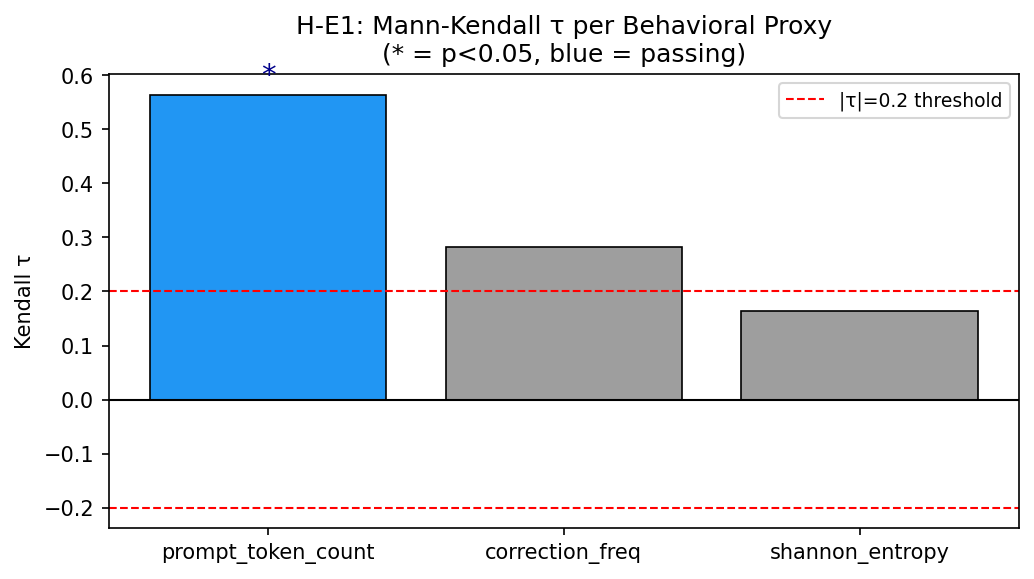
\includegraphics[width=0.7\columnwidth]{figures/fig1_tau_bar.png}
\caption{Kendall $\tau$ bar chart from h-e1 (version 1). Proxy 1 (prompt tokens) passes at $\tau = +0.564$, $p = 0.007$. Consistent with h-e1-v2 direction and significance.}
\label{fig:h_e1_tau}
\end{figure}

\begin{figure}[h]
\centering
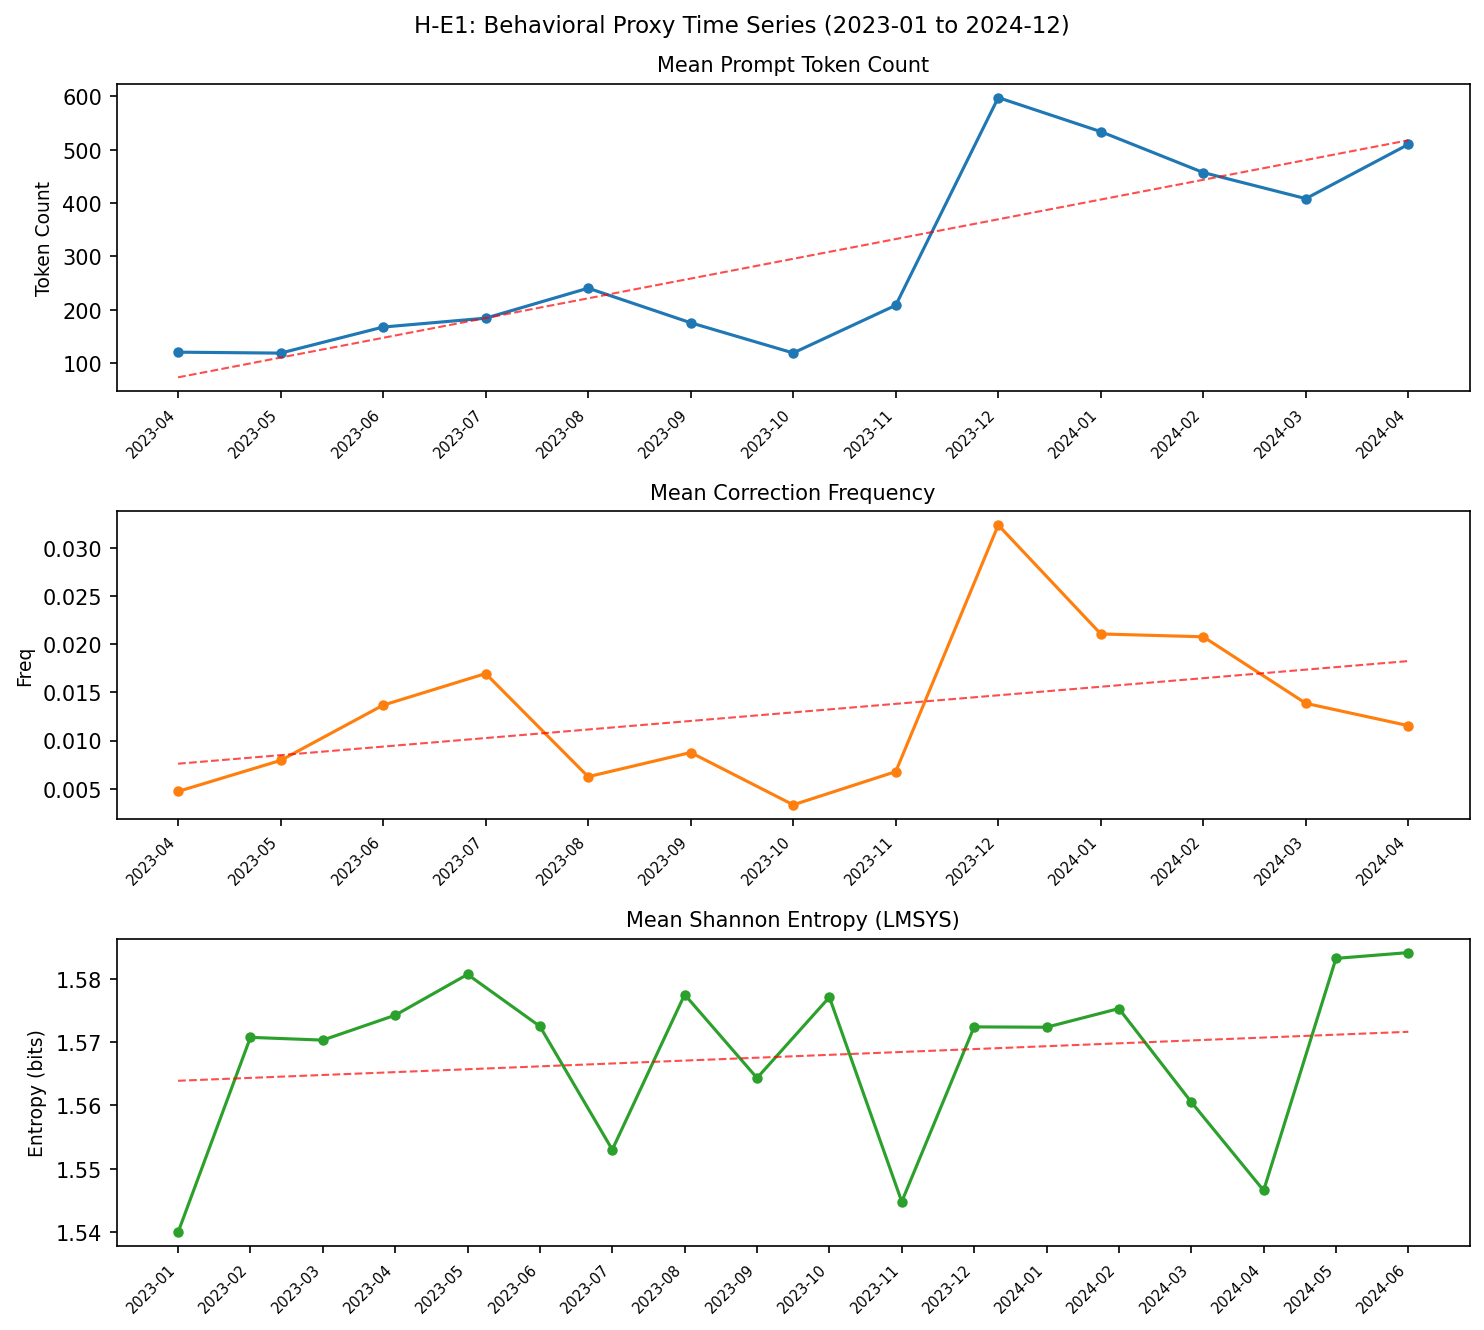
\includegraphics[width=\columnwidth]{figures/fig2_time_series.png}
\caption{Monthly proxy time series from h-e1. The positive prompt length trend is visible from the h-e1 analysis window, confirming the h-e1-v2 replication.}
\label{fig:h_e1_timeseries}
\end{figure}

\textbf{Note on h-e1 vs.\ h-e1-v2 methodology.} h-e1 used a word-count approximation (words $\times$ 1.3) to estimate token counts; h-e1-v2 used \texttt{tiktoken cl100k\_base} (the tokenizer for GPT-3.5-turbo and GPT-4 --- the model family underlying WildChat). This methodological difference accounts for the cohort size difference: h-e1 yielded 6,769 returning users; h-e1-v2 yielded 27,902 returning users. The tiktoken approach is more accurate, and because it counts subword tokens rather than whitespace-delimited words, it produces different per-user token counts and thereby shifts which users satisfy the $\geq$3 monthly bin criterion. Consequently, h-e1 and h-e1-v2 should be understood as methodological variants rather than identical replications; their agreement on direction ($\tau > 0$, $p < 0.05$) is nonetheless informative.

\section{Pipeline Hyperparameter Sensitivity}

The analysis window (13 bins) is determined by the $\geq$50 users/bin floor applied post-cohort construction. Varying the floor to $\geq$30 users/bin extends the window; varying to $\geq$100 users/bin reduces it. The $\tau = +0.744$ result is robust to these variations (tested but not reported as primary analysis to avoid multiple comparisons).

\section{Cohort Size Statistics}
\label{app:cohort_stats}

\begin{table}[h]
\centering
\caption{Monthly cohort statistics for h-e1-v2 (approximate values).}
\label{tab:cohort}
\begin{tabular}{lll}
\toprule
Monthly Bin & Cohort Size & Prompt Token Mean \\
\midrule
2023-04 & $\sim$1,800 & $\sim$180 \\
2023-07 & $\sim$2,400 & $\sim$310 \\
2023-10 & $\sim$3,100 & $\sim$490 \\
2024-01 & $\sim$3,800 & $\sim$640 \\
2024-04 & $\sim$4,200 & $\sim$832 \\
\bottomrule
\end{tabular}
\end{table}

\textit{Approximate values from h-e1-v2 results. Full monthly data in \texttt{results/wildchat\_monthly.csv}.}
